% --------------------------------------------------------------
% This is all preamble stuff that you don't have to worry about.
% Head down to where it says "Start here"
% --------------------------------------------------------------
 
\documentclass[11pt]{article}
 
\usepackage[margin=0.7in]{geometry} 
\usepackage{amsmath,amssymb}
\usepackage{hyperref}
\usepackage{amsfonts}
\usepackage{graphicx}
\graphicspath{ {./img/} }
\usepackage{hyperref}
\usepackage{algorithm2e}
\graphicspath{ {./} }

\usepackage{float}


\usepackage{tcolorbox}

 
\newtheorem{theorem}{Satz}
\newtheorem{acknowledgement}[theorem]{Acknowledgement}
\newtheorem{axiom}[theorem]{Axiom}
\newtheorem{case}[theorem]{Case}
\newtheorem{claim}[theorem]{Claim}
\newtheorem{conclusion}[theorem]{Conclusion}
\newtheorem{condition}[theorem]{Condition}
\newtheorem{conjecture}[theorem]{Conjecture}
\newtheorem{corollary}[theorem]{Corollary}
\newtheorem{criterion}[theorem]{Criterion}
\newtheorem{definition}[theorem]{Definition}
\newtheorem{example}[theorem]{Example}
\newtheorem{exercise}[theorem]{Exercise}
\newtheorem{lemma}[theorem]{Lemma}
\newtheorem{notation}[theorem]{Notation}
\newtheorem{problem}[theorem]{Problem}
\newtheorem{proposition}[theorem]{Proposition}
\newtheorem{remark}[theorem]{Remark}
\newtheorem{solution}[theorem]{Solution}
\newtheorem{summary}[theorem]{Summary}
\newenvironment{proof}[1][Beweis]{\textbf{#1.} }{\ \rule{0.5em}{0.5em}}
\begin{document}
 
% --------------------------------------------------------------
%                         Start here
% --------------------------------------------------------------
 
\title{Numerical Optimization - Homework 2}%replace X with the appropriate number
\author{Andy Tràn}
 
\maketitle %shows the current date of the Zusammenfassung
\section*{Problem 1}
\begin{enumerate}
    \item Let $g(x) = \mathbf{x}^T A \mathbf{x}$, $h(x) = \mathbf{x + b}$, then $f(x) = g(h(x))$. The gradient is $\nabla f(x) = h'(x)^T \nabla g(h(x)) = I \cdot (A+A^T)(\mathbf{x+b}) = (A+A^T)(\mathbf{x+b})$. $Hess_f(x) = A + A^T$ 
    \item $f(\textbf{x}) = \textbf{b}^T(A\textbf{x-y} ) = \textbf{b}^TA\textbf{x} - \textbf{b}^Ty$, thus $\nabla f(x) = A^T b $ and $Hess_f(x) = 0$ (zero matrix)  
    \item $f(x) = \left\lVert Ax - b\right\rVert^2 = (Ax-b)^T(Ax-b)$, let $h(x) = x^Tx $, $g(x) = Ax-b$. We have $ f(x) = h(g(x))$, thus $\nabla f(x) = g'(x)^T \cdot \nabla h(g(x)) = A^T \cdot 2 (Ax-b)$ and $Hess_f(x)=2A^TA$ 
    \item We can employ the chain rule by writing down, $h(x) = \sqrt(x), x\in \mathbb{R}$, and $g(x) = \left\lVert Ax-b\right\rVert^2$, thus $f(x) = h(g(x))$. Calculating $\nabla f(x) = \nabla g(x) \cdot h'(g(x)) = \frac{2A^T(Ax-b)}{2\left\lVert Ax-b\right\rVert }$. Now the harder part comes: \newline
    Let $\kappa(x) = \frac{1}{\left\lVert Ax - b\right\rVert }$ and $\tau(x) = A^T(Ax-b)$.We can write it as $\nabla f(x) = \tau(x) \kappa(x)$. Then we can employ the chain rule to calculate the derivative (Hessian). We can calculate these terms individually: 
    \begin{flalign*}
        Hess_f(x) &=  \tau(x) d \kappa(x) + d \theta(x)\kappa(x)\\
        &= A^T(Ax-b)\cdot -\frac{(x^TA^T-b^T)A}{\left\lVert Ax-b\right\rVert^3} + A^TA\cdot\frac{1}{\left\lVert Ax-b\right\rVert }\\
        &= \frac{A^TA}{\left\lVert Ax-b\right\rVert } - \frac{(A^TAx - b)((x^TA^T-b^T)A)}{\left\lVert Ax-b\right\rVert^3 }
    \end{flalign*}
\end{enumerate}


\section*{Problem 2 (Convex functions)}
\begin{itemize}
    \item Let's show $g_i(x) = | a_i^Tx + b_i|$ is convex for any vector $a_i$ and scalar $b_i$. Let those values be arb. but fix.
    \begin{flalign*}
        g_i(\lambda x + (1-\lambda)y) &= | a_i^T(\lambda x + (1-\lambda)y) + b_i |\\
        &= | a_i^T\lambda x + a_i^T(1-\lambda)y + b_i |\\
        &= | a_i^T\lambda x + \lambda b_i + a_i^T(1-\lambda)y + (1-\lambda)b_i |\\
        &\leq  | a_i^T\lambda x + \lambda b_i | + |a_i^T(1-\lambda)y + (1-\lambda)b_i |\\
        &= \lambda | a_i^Tx + b_i| + (1-\lambda) | a_i^T y + b_i |\\
        &= \lambda g_i(x) + (1-\lambda)g_i(y)
    \end{flalign*}
    
    Then the pointwise maximum is also convex, due to the theorem from the lecture.
    \item Firstly, we need to show $g(x)=x^3$ is convex on $[0, \infty[$, which is rather straightforward since we see $g''(x) = 6x \geq 0 \forall x \in[0,\infty[$ (and strictly positive for $x \neq 0$ ).We also need to show $h(x) = \left\lVert Ax - b\right\rVert$ is convex, which it is from the proposition from the slide where all norms are convex and functions composed with affine functions are also convex (else prove it quickly using the definition of convexity and triangle inequality). \begin{flalign*}
        f(\lambda v + (1-\lambda)w) &= g(h(\lambda v + (1- \lambda)w))\\
        &\leq g(h(\lambda v) + (1-\lambda)w)\\
        &\leq g(h(\lambda v)) + g(h((1-\lambda)w))\\
        & = f(\lambda v) + f((1-\lambda)w)
    \end{flalign*}
    The first inequality follows from the convexity of $h(x)$ and the second from convexity of $g(x)$. 
    
    \item In the previous step (2) we proved $\left\lVert A\mathbf{x +b}\right\rVert^3  $ is convex, we need to prove $h(x) =e^x$ is convex as well for any x. The derivatives $h'(x)=h''(x) = e^x$ show us that $h'(x)$ is always increasing and $h''(x)$ shows us $e^x$ is convex as well. Employing the composition rule from the lecture, $f(x) = h(\left\lVert A\mathbf{x +b}\right\rVert^3 )$ is convex as well due to the inner function also being non-decreasing.
    
    \item We can define new auxillary functions, namely $g_i(x) = a_i^T x$, where $a_i$ is a vector where $k$ values are set to 1 and all the other values are 0. We have $\binom{n}{k}$ of these vectors. We can redefine $f(x) = \underset{i}{\max}g_i$. All there is left to show is that $g_i(x) = a_i^T x $ is convex as well. Namely, let $g_i(x)$ be arb. but fix
    
    \begin{flalign*}
        g_i(\lambda x + (1-\lambda)y) &= a_i^T (\lambda x + (1- \lambda)y)\\
        &= a_i^T \lambda x + a_i^T (1-\lambda)y\\
        &= \lambda g_i( x) + (1-\lambda)g_i(y)
     \end{flalign*}
     which concludes our proof combined with the proposition that a pointwise maximum is also convex.
\end{itemize}


\section*{Problem 3}
\begin{enumerate}
    \item \textbf{Proof:} let $S_f(t) = \{ x \in dom(f) : f(x) \leq t \}$. We want to prove over the definition, namely $x,y \in S_f(t)$, then for $\theta \in [0,1]: \theta x + (1-\theta)y \in S_f(t)$
    \newline
\textbf{    Case Distinction:
}     \begin{enumerate}
        \item Let $\theta = \{0,1\}$, then it immediately follows $\theta x + (1-\theta)y = x \in S_f(t)$, conversely for $\theta = 0$ 
        \item Let $\theta \in ]0,1[$ and case distinction over $x\leq y$ and $x > y$. We do the second case and the other one should be immediately clear. \[
        \theta x + (1-\theta)y < \theta x + (1-\theta)x = x
        .\]     
    \end{enumerate} and as follows we have due to $x \leq y \Rightarrow \sqrt{x} \leq \sqrt{y}$ following $\sqrt{\theta x + (1-\theta)y} < \sqrt{x} \leq t$, which concludes our proof.  
    
    \item This can be easily proven over the definition. Let $f(x)$ be convex such that $f(\theta x + (1-\theta)y) \leq \theta f(x) + (1-\theta)f(y)$ and let it's sublevel set $S_f(t) = \{ x \in dom(f) : f(x) \leq t \}$. We want to show $x,y \in S_f(t)$, then for $\theta \in [0,1]: \theta x + (1-\theta)y \in S_f(t)$. 
    
    We can show this as follows:
    \begin{flalign*}
        f(\theta x + (1-\theta)y) &\leq \theta f(x) + (1-\theta)f(y)\\
        &\leq \theta t + (1-\theta)t\\
        &= t
    \end{flalign*}

    Where the second inequality follows from $x\in S_f(t) \Rightarrow f(x) \leq t$ 
       
    \item \begin{enumerate}
        \item We must show $f(x) = |x+b|^p$ is quasi convex for $p\in]0,1[$, since from the lecture we know it's convex for $p \geq 1$. Also the inequality $x \leq y \Rightarrow |x|^p \leq |y|^p$ for $p \in ]0,1[$ (can be shown with the first derivative always being $>$ 0, except for the point where the argument is 0, thus monotonically increasing) allows us to reuse the proof from (1). This altogether show its sublevel set is also convex.
        \item This one was one of the harder proof, but nonetheless we can attempt it :) and didn't work for me over the defintion so we cheat a little bit here. We know from the lectures half-spaces $H = \{\mathbf{x} : \mathbf{a}^T\mathbf{x} \leq k \}$ are convex. So if we look at the sublevel set $S_f(t) = \{ \mathbf{x} \in dom(f): f(x) \leq t \} = \{\mathbf{x} : \frac{a^Tx + b}{c^Tx + d} \leq t \} = \{\mathbf{x} : a^Tx + b \leq t(c^Tx + d) \} = \{\mathbf{x} : (a^T-t c^T) x\leq dt - b \}$. Which is a halfspace, and thus convex.
        
    \end{enumerate}
    
    \item \begin{enumerate}
        \item Analyzing the second derivative $f''(x)= p \cdot (p-1)|x+b|^{p-2}$, shows us that $f''(x) < 0 \forall x\neq 0$. At all those points it's concave down and we have showed it's not convex.  
        \item We can take an counterexample, let $(a,b,c,d) = (1, 0, 1, 0)$ and $x = [u, \sqrt{u}]^T$, which gives $f(x) = \frac{u}{\sqrt{u}} = \sqrt{u}$, which is a concave function, given $u \geq 0$. This can be easily proven with going over the definition of a concave function $f(\theta x + (1-\theta)y) > \theta f(x) + (1-\theta)f(y)$       
    \end{enumerate}
    
    
\end{enumerate}

\section*{Problem 4}
\begin{enumerate}
    \item \begin{flalign*}
        \frac{df(z)}{dz} &= \frac{(e^z + e^{-z})(e^z + e^{-z}) - (e^z - e^{-z})(e^z - e^{-z})}{(e^z + e^{-z})^2}\\
        &= 1 - \frac{(e^z - e^{-z})^2}{(e^z + e^{-z})^2}\\
        &= 1- \tanh^2(z)
    \end{flalign*}

    and for the second derivative we can calculate:

    \[
    \frac{d^2f(z)}{dz^2} = -2 [\tanh(z)]' \tanh(z) = -2 (1- \tanh^2(z)) \tanh(z)
    .\] 
            
    \item Solution:
    \begin{figure}[H]
        \centering
        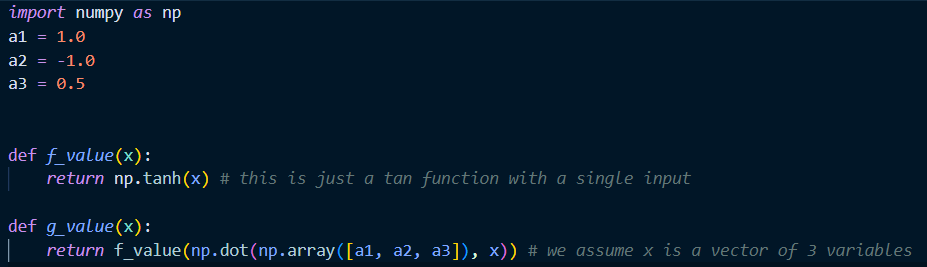
\includegraphics[width=0.7\textwidth]{part2.png}
        \label{fig: subq2}
    \end{figure}
    \item Solution:
    \begin{figure}[H]
        \centering
        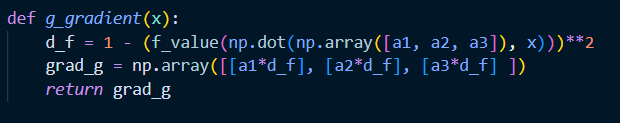
\includegraphics[width=0.7\textwidth]{part3.png}
        \label{fig: subq3}
    \end{figure}
    \item Solution:
    \begin{figure}[H]
        \centering
        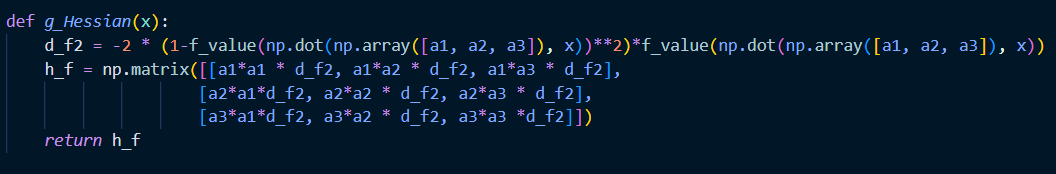
\includegraphics[width=0.7\textwidth]{part4.png}
        \label{fig: subq4}
    \end{figure}
    
\end{enumerate}




\end{document}